\chapter{Bute: A Bottom-Up Algorithm for Treedepth}
\label{c:bute}

\section{THE ALGORITHM}

\subsection{Optimisation as a sequence of decision problems}

Algorithm \ref{alg1} takes as input a connected graph $G$ and returns the treedepth of $G$.
In common with the existing implemented approaches to solving the problem, the algorithm solves
a sequence of decision problems.  We work upwards: for $d=1, 2,\dots$, the algorithm
solves the decision problem of whether $G$ admits an elimination tree of depth no greater than $d$.
The algorithm returns $d$ after solving the first satisfiable decision problem.

\Lineref{callHeurFunc} calls a heuristic function to obtain an upper bound on the treedepth of
$G$.  This call is advantageous only in the case where the heuristic returns the treedepth
of $G$.  In this case, the call to $\FuncSty{decomposition\_exists}(G, d)$ on line \codelineref{callSolveFunc}
with $d = \td(G)$---that is, the first call to the decision problem that returns $\AlgVar{true}$---can be avoided.

The simplest possible version of $\FuncSty{heur\_upper\_bound}(G)$ simply returns $|V(G)|$.
The version of $\FuncSty{heur\_upper\_bound}$ that we use in our implementation uses a portfolio
of heuristic solvers and repeated tries to replace a subtree of an elimination tree with an improved
subtree on the same vertex set; wee will be described this in more detail later.

{
\begin{algorithm}[htb]
 \footnotesize
\DontPrintSemicolon
\newcommand\solveFn{\FuncSty{decomposition\_exists}}
\newcommand\optimiseFn{\FuncSty{optimise}}
\newcommand\true{\AlgVar{true}}
\newcommand\false{\AlgVar{false}}

\nl $\optimiseFn(G)$ \label{dummylabel} \;
\nl \KwData{Connected graph $G$}
\nl \KwResult{The treedepth of $G$}
\nl \Begin{
  \nl $b \gets \FuncSty{heur\_upper\_bound}(G)$ \; \label{callHeurFunc}
  \nl \For{$d\gets 1, \dots, b-1$} {
  \nl   \If{$\solveFn(G, d)$} { \label{callSolveFunc}
  \nl     \KwSty{return} $d$ \;
      }
  }
  \nl \KwSty{return} $b$ \;
}
\caption{The $\optimiseFn$ function of the Bute algorithm}
\label{alg1}
\end{algorithm}
}

\FloatBarrier

\subsection{Solving the decision problem}

Algorithm \ref{alg2} solves the decision problem of whether graph $G$ admits a treedepth decomposition of
depth at most $k$.
\Lineref{initialiseU} and \linerangeref{opt1}{updateU} are optimisations that can be ignored
on an initial reading; they will be described later in this section.

{
\begin{algorithm}[htb]
 \footnotesize
\DontPrintSemicolon
\newcommand\target{\AlgVar{target}}
\newcommand\solveFn{\FuncSty{decomposition\_exists}}
\newcommand\optimiseFn{\FuncSty{optimise}}
\newcommand\true{\AlgVar{true}}
\newcommand\false{\AlgVar{false}}

\nl $\solveFn(G, k)$ \;
\nl \KwData{Connected graph $G$, natural number $k$ such that $\td(G) \geq k$}
\nl \KwResult{$\true$ if and only if $G$ has treedepth less than or equal to $k$}
\nl \Begin{
  \nl $\calS \gets \emptyset$ \;
  \nl $\calU \gets \emptyset$ \;  \label{initialiseU}
  \nl \For{$i\gets k; i \geq 1; i \gets i - 1$} {  \label{iLoop}
      \nl $\calS \gets \MakeSTSs(G, \calS, i)$ \;  \label{makeS}
      \nl \lIf{$\calS \subseteq \calU$}{\KwSty{return} $\false$}  \label{opt1}
      \nl \For{$S \in \calS$ \label{opt2start}} {
          \nl \lIf{$|S| + |N(S)| = n$}{\KwSty{return} $\true$} \label{opt2end}
      }
      \nl $\calU \gets \calU \cup \calS$ \;  \label{updateU}
   }
   \nl \lIf{$\calS \not= \emptyset$}{\KwSty{return} $\true$}
   \nl \lElse{\KwSty{return} $\false$}
}
\caption{The $\solveFn$ function of the Bute algorithm}
\label{alg2}
\end{algorithm}
}

Our strategy will be to generate, for each value of $i$ from $k$ down to 1, a collection of sets $\calS_i^k$.
Collection $\calS_i^k$ contains the vertex set of each subtree whose root is at depth $i$ of
some depth-$k$ elimination tree of $G$.
For $1 \leq i \leq k$, we define
$\calS_i^k$ to be the set of subsets $S$ of $V(G)$ such that (1) $G[S]$ admits an elimination tree
of depth at most $k-i+1$, (2) $|N(S)| < i$, and (3) the subgraph of $G$ induced by $S$
is connected.  For any elimination tree $T$ of depth
$k$ and any subtree $T'$ rooted at depth $i$ of $T$, we have $V(T') \in \calS_i^k$ (as I will
prove in a later draft).  The converse is not true; $\calS_i^k$ may contain a set of vertices that
is not the vertex set of any subtree of an elimination tree of $G$.  This does not affect the correctness
of the algorithm, but our hope is that $\calS_i^k$ is defined sufficiently narrowly that the collection
of sets of vertices generated is fairly small.

In the terminology of Tamaki \cite{DBLP:journals/jco/Tamaki19}, the elements of the
$\calS_i^k$ are \emph{positive instances}. Each set satisfies a necessary condition for
being the vertex-set of a subtree whose root is at depth $i$ of the elimination tree.
The algorithm proceeds by combining positive instances into larger positive instances; each set in
the collection $\calS_i^k$ is created by combining zero or more sets from $\calS_{i+1}^k$ with an
additional vertex in the function $\MakeSTSs$; the next section will describe this function in detail.

\Lineref{makeS} calls the function
$\MakeSTSs$ to create $\calS_i^k$ for each value of $i$ from $k$ down to $1$.  After the loop terminates,
the variable $\calS$ holds the collection $\calS_1^k$.  The function then returns $\AlgVar{true}$ if and only
this collection is non-empty.\footnote{I will prove that a non-empty $\calS_1^k$ is a necessary and sufficent
condition of $G$ admitting an elimination tree of depth $k$.}

The function has two optimisations which may be omitted without affecting the function's correctness.  For
the first of these optimisations, all sets of vertices seen so var in the $\calS$-collections are added to
a collection $\calU$.  On \codelineref{opt1}, the function returns $\AlgVar{false}$ if $\calS_i^k$ does
not contain any set that has not already appeared in some $\calS_j^k$ with $j>i$.\footnote{I will also
need to prove that this optimisation is valid and demonstrate that it is useful.  The usefulness
can be shown experimentally. The argument for correctness
is as follows: We assume that $G$ has treedepth at least $k$ (this precondition to the function
is satisfied because we optimise by a sequence of decision problems with ascending $k$).
Since every member of $\calS_i^k$
is also in $\calS_j^k$ for some j>i, it must be case that for each $S \in \calS_i^k$, $G[S]$ admits
an elimination tree of depth at most $k-i$.  Now let $T$ be some depth-$k$ elimination tree of $G$.
We can replace each subtree of $T$ whose root is at depth $i$ with a subtree on the same vertex set
with depth at most $k-i$, giving a treedepth decomposition of $G$ of depth at most $k-1$.
This contradicts our assumption that $G$ has treedepth at least $k$.}

The second optimisation is on \linerangeref{opt2start}{opt2end}.  This returns $\AlgVar{true}$ if
there is some $S \in \calS$ such that the union of $S$ and its neighbourhood comprises the vertex set
of $G$.  If this is the case, a treedepth decomposition $T$ can be formed trivially by placing one
vertex of $N(S)$ at each depth of the tree from depth $1$ to depth $|N(S)|$, then adding a minimum-depth
elimination tree of $G[S]$ as the unique subtree of $T$ whose root is at depth $|N(S)| + 1$.\footnote{I
will add a figure illustrating this.  I will also give a way to produce an \emph{elimination tree} rather
than merely a treedepth decomposition using this approach.  This just requires removing the vertices of $N(S)$
from $G$ one by one in an order than leaves the remainder of $G$ connected.  It is straightforward to do:
just list the vertices of $N(S)$ in reverse order of distance from $S$ in $G$.}

\FloatBarrier

\subsection{The $\MakeSTSs$ function}

Algorithm \ref{ConstructingTheS} is copied from an old draft and is not yet complete.
It doesn't include all the implemented optimisations and may have bugs, but I'm including
this version just to show an outline of the approach.
I have written a draft of pseudocode for this part of the algorithm with pen and paper,
but have not yet typed it up.

The function $\MakeSTSsHelper$ performs a backtracking search to create all elements of
$\calS_i^k$.  Each element comprises a vertex $v$ and a (possibly empty) subset $S$ of $\calS_{i+1}^k$
such that:

\begin{itemize}
  \item $v$ is not in any member of $S$.
  \item The sets in $S$ are pairwise disjoint.
  \item There do not exist $A, B \in S$ such that $u$ and $w$ are adjacent in $G$ for some
        $u \in A$ and $w \in B$.
  \item $v$ is adjacent to at least one vertex in each member of $S$.
  \item $|N_G(\{v\} \cup \bigcup S)| < i$.
\end{itemize}

(I will prove that these conditions are jointly necessary and sufficient for membership in $\calS_i^k$---I
think the proof is quite easy.)

(The tricky part will probably be proving that the function is correct.  The way it branches is
quite similar to a standard clique algorithm (e.g. MCSa1), so I think the proof won't be \emph{too}
tricky. I will also need to think about explaining my choices for variable ordering and filtering.
For variable ordering, I have implemented two options, and I should probably compare them experimentally. The domain
filtering (in CP terminology, although I don't think I'll use that terminology here) probably doesn't
achieve any standard level of consistency, so I don't know if there's much that I can say about it
other than perhaps pointing out ways in which more filtering could be done at the cost of extra
time per recursive call.)

{
\begin{algorithm}[htb]
 \footnotesize
\DontPrintSemicolon
\newcommand\target{\AlgVar{target}}
\newcommand\true{\AlgVar{true}}
\newcommand\false{\AlgVar{false}}

\nl $\AddSubtreeRoot(\calG, i, R, U, \calS_{out})$ \;
\nl \KwData{Connected graph $\calG$, natural number $i$,
        set of vertices $R$ (possible roots of subtree), set of vertices $U$
        (union of vertices of child subtrees), set of sets of vertices $\calS_{out}$}
\nl \KwResult{Updated $\calS_{out}$, including all permissible STSs whose set
        of non-root vertices equals $U$}
\nl \Begin{
    \nl \For{$v \in R$} {
        \nl $S \gets U \cup \{v\}$ \;
        \nl \If{$|N(S)| \leq i$ TODO: make code like this} {
            \nl $\calS_{out} \gets \calS_{out} \cup \{S\}$\;
        }
    }
    \nl \Return $\calS_{out}$ \;
}

\vspace{1em}

\nl $\MakeSTSsHelper(\calG, \calS, i, R, U, \calS_{out})$ \;
\nl \KwData{Connected graph $\calG$, set of sets of vertices $\calS$ (stored as an array), natural number $i$,
        set of vertices $R$ (possible roots of subtree), set of vertices $U$
        (union of vertices of child subtrees), set of sets of vertices $\calS_{out}$}
\nl \KwResult{An updated $\calS_{out}$ including all subtree-sets whose non-root
        vertices consist of the union of $U$ and a union of members of $\calS$}
\nl \Begin{
  \nl $\calS' \gets \emptyset$ \Comment{$\calS'$ is stored as an array} \label{MakeSPrime} \;
  \nl \ForEach{$S \in \calS$\label{SLoop}} {
      \nl $U' \gets U \cup S$ \Comment{comment}\;
      \nl $R' \gets R \cap N(S)$ \Comment{comment}\;
      \nl $\calS_{out} = \AddSubtreeRoot(\calG, R', U', \calS_{out})$ \label{CallAddSubtreeRoot} \;
      \nl $\calS_{filtered} \gets \{S' \in \calS' : |N(S') \cup N(U')| \leq i
            \wedge N(S') \cap R' \not= \emptyset \wedge N[U'] \cap S' = \emptyset\}$ \label{FilterSTSs} \;
      \nl $\MakeSTSsHelper(\calG, \calS_{filtered}, i, R', U', \calS_{out})$ \;
      \nl $\calS' \gets \calS' \cup \{S\}$ \label{AddToSPrime} \;
  }
}

\vspace{1em}

\nl $\MakeSTSs(\calG, \calS, i)$ \;
\nl \KwData{Connected graph $\calG$, set of sets of vertices $\calS=\calS_{i+1}^k$, natural number $i$}
\nl \KwResult{The set $\calS_i^k$}
\nl \Begin{
    \nl $\calQ \gets \{\{v\} \mid v \in V(\calG) \wedge |N(v)| < i\}$ \;
    \nl $\calR \gets \MakeSTSsHelper(\calG, \calS, i, V(\calG), \emptyset, \emptyset)$ \label{FirstHelperCall} \;
    \nl \Return $\calQ \cup \calR$
}
\caption{Constructing the set $\calS_i^k$.  TODO: make this and other captions more useful to the reader}
\label{ConstructingTheS}
\end{algorithm}
}

\section{Notes to self}

TODO: Cite Bannach and Berndt.  Maybe run a draft of the paper I'm writing past them?
My algorithm seems similar to their PACE Challenge 2020 entry.  Are the main differences in
how they are described and the fact that I use a trie?

TODO: Cite \cite{DBLP:journals/algorithmica/FominGP15}.  My basic algorithm is possibly
very close to their basic DP algorithm.  This approach also possibly suggested in the
Sparsity book.

\section{Introduction}

This paper presents \emph{Bute}, a new algorithm for the exact treedepth problem.
A \emph{treedepth decomposition} of a graph $G$ is a forest $F$ on the vertices
of $G$, such that any pair of vertices that are adjacent in $G$ have an ancestor-descendant
relationship in $G$.  The treedepth problem is, given graph $G$, to find the minimum depth of a 
treedepth decomposition of $G$.

Our algorithm constructs a minimum-depth \emph{elimination tree}, using the well-known
result that the minimum depth of an elimination tree of $G$ equals the treedepth of $G$.
We only consider connected graphs as input.  The concept of elimination tree generalises
naturally to \emph{elimination forest} for connected graphs (define it).
An elimination tree of connected graph $G$ is constructed as follows.  If $G$ has
a single vertex, its elimination tree is a single-vertex tree with vertex
set $\{v\}$.  Otherwise, remove a vertex
$v$ and its incident edges from $G$, and make this the root of the tree.  
Make an elimination tree of each component and make these child subtrees
of $v$.
TODO: prove that bottom-up definition is equivalent.  Give a citation?

Mention previous DP algorithms.  $2^n$ algorithm (suggested by N and dm M?).
$1.96^n$ algorithm.

Prior implementations of exact algorithms for treedepth:
two SAT encodings by Ganian et al.\ \cite{DBLP:conf/alenex/GanianLOS19,DBLP:journals/corr/abs-1911-12995},
James's top-down algorithm that branches on roots of subtrees \cite{DBLP:conf/wea/000120a}.

Exact treedepth was one of the two tracks of the 2020 PACE Challenge. The algorithm
described here is a slightly cleaned-up version of a solver submitted
to the challenge.

The algorithm we present solves the problem from the bottom up, by finding sets
of vertices that induce subgraphs of small treedepth.  I think that it's a positive-instance
driven (PID) dynamic programming algorithm \cite{DBLP:journals/jco/Tamaki19}, but I don't yet
understand the Tamaki paper well enough to be sure.  Bannach and Berndt \cite{DBLP:conf/wads/BannachB19}
outline a PID approach to treedepth but don't implement it (although they have subsequently
implemented a version of it for the PACE Challenge). So I need to figure out to what extent
I've reinvented their idea.

\subparagraph*{Outline of the paper.}  \Cref{sec:preliminaries} introduces notation.
\Cref{sec:algorithm} presents our algorithm.  \Cref{sec:trie} describes the trie data structure
that is important for the performance of our algorithm.  \Cref{sec:improvements} describes
improvements to the algorithm.  \Cref{sec:implementation} describes low-level implementation details.
\Cref{sec:paceentries} discusses other entries to the PACE Challenge 2020, based on a quick
look at their code and two-page descriptions.  \Cref{sec:experiments} presents our experiments,
and \Cref{sec:conclusion} concludes.




\section{Preliminaries}\label{sec:preliminaries}

This section introduces notation, followed by two simple propositions about elimination trees
on which our algorithm is based.

\subsection{Notation}

\subparagraph*{Graphs.} We write $V(G)$ and $E(G)$ to denote the vertex and edge sets of a graph $G$.
The subgraph of $G$ induced by a set $S \subseteq V$, written $G[S]$, is the graph
$(S, \{\{u,v\} \in E \mid u,v \in S\})$.

TODO: be consistent about what a component is.  Is it a set of vertices or a subgraph?

The \emph{neighbourhood} $N_G(v)$ of a vertex $v$ is the set of vertices adjacent to $v$
in $G$.
The \emph{closed neighbourhood} $N_G[v]$ of $v$ is $N_G(v) \cup \{v\}$.
We define these operators on sets of vertices also:
for $S \subseteq V$, we have $N_G(S) = \bigcup_{v \in S}{N_G(v)} \setminus S$
and $N_G[S] = N_G(S) \cup S$.
Where the context makes clear which graph we are referring
to, we omit the subscript of the neighbourhood operators.


\subparagraph*{Trees.} All trees in this paper are rooted.  We say that the root of a tree is at depth 1,
its children are at depth 2, and so on.  The depth of a tree is the depth equals
the depth of its deepest vertex.

The treedepth of a graph $G$ is denoted by $td(G)$.  Recall that this is equal to the
minimum depth of an elimination tree of $G$.

We write $T[v]$ or $T_v$ to denote the subtree of $T$ rooted at $v$.  TODO use consistent notation
throughout; choose $_v$ probably.

\subparagraph*{Strong disjointness.} Finally, we introduce the following
definition which will be useful for describing a property of elimination trees.
Let $U,W \subseteq V(G)$ such that $U \cap N_G[W] = \emptyset$; that is, $U$
and $W$ are disjoint and there is no edge $\{u,w\} \in E(G)$ such that $u \in
U$ and $w \in W$.  We say that $U$ and $W$ are \emph{strongly disjoint} in $G$.

\subsection{An alternative definition of elimination tree}

\begin{figure}[htb]
  \centering
\begin{tikzpicture}[scale=0.85,
        every node/.style={circle,draw=black,inner sep=2pt,scale=0.85}]
    \node (1) at ( 0.0, 1.2) {1};
    \node (2) at ( 0.8, 0.65) {2};
    \node (3) at ( 0.5,-0.3) {3};
    \node (4) at (-0.5,-0.3) {4};
    \node (5) at (-0.8, 0.65) {5};
    \node (6) at (-1.6, 0.65) {6};
    \node (7) at (-0.7, 1.9) {7};
    \node (8) at ( 0.0, 2.6) {8};
    \node (9) at ( 0.7, 1.9) {9};
    \node[draw=none] () at (0,-.7) {};   % just to move the picture up a bit

    \draw (1) -- (2) -- (3) -- (4) -- (5) -- (1);
    \draw (5) -- (6);
    \draw (1) -- (7) -- (8) -- (9) -- (1);
    \draw (1) -- (8);
    \draw (7) -- (9);

\end{tikzpicture}
\qquad\qquad
\begin{tikzpicture}[scale=0.85,
        every node/.style={circle,inner sep=2pt,scale=0.85}]
    \node (1) at (1.5,2.4) {1};

    \node (7) at (.6,1.6) {7};
    \node (4) at (2.4,1.6) {4};

    \node (8) at (.6,0.8) {8};
    \node (9) at (.6,0) {9};
    \node (5) at (1.8,0.8) {5};
    \node (6) at (1.8,0) {6};
    \node (2) at (3.0,0.8) {2};
    \node (3) at (3.0,0) {3};

    \draw (1) -- (7) -- (8) -- (9);
    \draw (1) -- (4) -- (5) -- (6);
    \draw (4) -- (2) -- (3);
    \node[draw=none] () at (0,-.8) {};   % just to move the picture up a bit
\end{tikzpicture}
\qquad\qquad
\begin{tikzpicture}[scale=0.85,
        every node/.style={circle,inner sep=2pt,scale=0.85}]
    \node (1) at (1.5,2.1) {1};

    \node (7) at (.6,1.4) {7};
    \node (4) at (2.4,1.4) {4};

    \node (8) at (.6,0.7) {8};
    \node (9) at (.6,0) {9};

    \node (5) at (2.4,0.7) {5};
    \node (6) at (2.4,0) {6};
    \node (2) at (2.4,-0.7) {2};
    \node (3) at (2.4,-1.4) {3};

    \draw (1) -- (7) -- (8) -- (9);
    \draw (1) -- (4) -- (5) -- (6) -- (2) -- (3);
\end{tikzpicture}

  \caption{An example graph $G$ and two treedepth decompositions of $G$.  The first decomposition has
  depth 4 and is an elimination tree; the second decomposition has depth 6 and is not an elimination tree.}
  \label{fig:example-graph}
\end{figure}

\begin{proposition}\label{elimination-tree-position}
Let $G=(V,E)$ be a connected graph and let $T$ be a treedepth decomposition of $G$. Tree $T$
is an elimination tree of $G$ if and only if $G[V(T_v)]$ is connected for each $v \in V$.
\end{proposition}

\begin{proof}
In this proof, we write \emph{connected treedepth decomposition (CTDD)} of $G$
to denote a treedepth decomposition $T$ of $G$ with the property in the proposition:
that $G[V(T_v)]$ is
connected for each $v \in V(G)$.  We need to show that a tree $T$ is an
elimination tree of connected graph $G$ if and only if $T$ is a CTDD of $G$.


(elimination tree $\Longrightarrow$ CTDD) Suppose we have a connected graph $G$
and an elimination tree $T$ of $G$ which is not a CTDD of $G$.  Let $v, w \in
V(G)$ be vertices such that the following three conditions hold: $w$ is the
parent of $v$ in $T$; $G[V(T_v)]$ is disconnected; and $G[V(T_w)]$ is
connected.  (We can find such a $v$ by starting at any vertex $u$ such that
$G[V(T_u)]$ is disconnected and letting $v$ be the furthest ancestor of
$u$ in $T$ such that $G[V(T_v)]$ is disconnected.  Since $G$ is connected,
$v$ must have a parent in the elimination tree.)  Since $T_w$ is an elimination
tree, $G[V(T_v)]$ is a connected component of $G[V(T_w)] - w$.   This contradicts
our assumption that $G[V(T_v)]$ is disconnected.

(CTDD $\Longrightarrow$ elimination tree)
We prove this implication by induction on $n$, the number of vertices in $G$.
The base case $n=1$ is trivial.  For the inductive case, let $n>1$ be given
and assume that for all $n' < n$ we have that every CTDD of an $n'$-vertex
connected graph is also an elimination tree of the graph.  Let $G$ be an $n$-vertex
connected graph and let $T$ be a CTDD of $G$.

We will show that $T$ is an elimination tree of $G$; to do this, it suffices
to show for each depth-2 vertex $w$ of $T$ that the vertex set of
$T_w$ is a connected component of $G[V(G)\setminus\{v\}]$, where $v$ is the root of $T$.  Since $T$ is a
CTDD, the vertex set of each $T_w$ must be a subset of one of these connected
components.  It remains to show that there is no depth-2 vertex $w$ in $T$ such
that $T_w$ is a proper subset of one of the connected components of
$G[V(G)\setminus\{v\}]$.  Suppose, for contradiction, that one of the $T_w$ is
a proper subset of a component $C$ of $G[V(G)\setminus\{v\}]$. Then there exist
vertices $t, u$ in $C$ such that $t$ is in $T_w$ and $u$ is in the
subtree rooted at a depth-2 vertex other than $w$.  Since $C$ is
connected, there must be a path from $t$ to $u$ in $G$.  Some edge
along this path must have one endpoint in $V(T_w)$ and one endpoint outside
$V(T_w)$.  These two endpoints do not have an ancestor-descendant relationship
in $T$, contradicting the assumption that $T$ is a treedepth decomposition of
$G$.
\end{proof}

\emph{Notes to self: I haven't seen the CTDD concept in the literature, but I need to search
more thoroughly.  There is a paper that uses a type of elimination tree that is guaranteed
to be a CTDD.  Sparsity book seems to have an incorrect lemma that is cited by Tamaki
and coauthor?}

\subsection{Properties of elimination trees}

This section introduces two very simple propositions about elimination trees
that will be used to show the correctness of our algorithm.  The first
proposition gives two simple properties that hold for any subtree of an
elimination tree.  TODO: give some intuition here about the role of these
propositions in the rest of the paper.

\begin{proposition}\label{subtreeproposition}
Let $G$ be a connected graph, and let $T$ be an elimination tree of $G$ of depth $k$.  For any $i \in \{1, \dots, k\}$
and any subtree $T'$ whose root is at depth
$i$ of $T$, the following three properties hold: (1) $T'$ has depth at most $k-i+1$, (2) $|N(V(T'))| < i$,
and (3) the subgraph of $G$ induced by $V(T)$ is connected.
\end{proposition}
\begin{proof}
The first property is trivial, since if it did not hold $T$ would have depth greater than $k$.

The second property holds because each vertex in $N(V(T'))$ must appear on the path
in $T$ from the root of $T$ to the root of $T'$; otherwise, there would exist some $v \in V(T')$
and some $v' \in N(V(T'))$ adjacent to $v$ such that $v$ and $v'$ do no have an ancestor-descendant
relationship in $T$.  This would mean that $T$ is not a treedepth decomposition, and hence
that it is not an elimination tree.

The third property follows from the definition of an elimination tree.
\end{proof}

\begin{proposition}\label{joiningETproposition}
Let $G$ be a connected graph, and let $T$ be an elimination tree of $G$.  Let $v$ be the root of $T$,
and let $T'$ and $T''$ be distinct child subtrees of $v$ in $T$.  Then
$V(T')$ and $V(T'')$ are strongly disjoint in $G$.
\end{proposition}
\begin{proof}
For each $v \in v(T')$, we have that $v \not\in V(T'')$, because otherwise
$v$ would appear twice in $T$.  Furthermore, $v \not\in N_G(V(T''))$; otherwise, there would
be some $w \in V(T'')$ adjacent to $v$ in $G$ such that $v$ and $w$ do not have an ancestor-descendant
relationship in $T$; this violates the definition of a treedepth decomposition.
\end{proof}



\section{The Bute algorithm}\label{sec:algorithm}

This section begins by describing the basic structure of the Bute algorithm.  We then
give a example of the algorithm's operation on a small input graph, and describe how the
algorithm can be easily modified to output a minimum-height elimination tree rather than
merely a single number.

\subsection{An outline of the algorithm}

\subparagraph*{Optimisation as a sequence of decision problems.}
Our algorithm takes as input a connected graph $\calG$ and returns the treedepth of $\calG$.
In common with the existing implemented approaches to solving the problem, the algorithm solves
a sequence of decision problems.  We work upwards: for $k=1, 2,\dots$, the algorithm
solves the decision problem of whether $\calG$ admits an elimination tree of depth no greater than $k$.
The algorithm returns $k$ after the first satisfiable decision problem.

\subparagraph*{Candidate vertex sets of subtrees.}
For $1 \leq i \leq k$, we define
$\calS_i^k$ to be the set of subsets $S$ of $V(G)$ such that (1) $G[S]$ admits an elimination tree
of depth at most $k-i+1$, (2) $|N(S)| < i$, and (3) the subgraph of $G$ induced by $S$
is connected.
It is clear from \Cref{subtreeproposition} that for any elimination tree $T$ of depth
$k$ and any subtree $T'$ rooted at depth $i$ of $T$, we have $V(T') \in \calS_i^k$.

In the terminology of Tamaki \cite{DBLP:journals/jco/Tamaki19}, the elements of the
$\calS_i^k$ are \emph{positive instances}. Each set satisfies a necessary condition for
being the vertex-set of a subtree whose root is at depth $i$ of the elimination tree.

%It is useful to think of each element $S \in \calS_i^k$ as representing a
%minimum-depth elimination tree of $G[S]$ which is being considered as a candidate subtree
%rooted at depth $i$ of an elimination tree of $G$.  Indeed, one could imagine a minor
%(and indeed slightly more intuitive) variation
%of our algorithm in which the elements of each $\calS_i^k$ \emph{are} elimination trees,
%and these are combined in a bottom-up fashion to form an elimination tree of $G$.
%The advantage of our approach using sets of vertices is that $G[S]$ may may admit many
%elimination trees of minimum depth, and it is sufficient to only consider one of these
%elimination trees as a candidate subtree for the elimination tree of $G$.

\subparagraph*{Constructing the $\calS_i^k$ in sequence.}
The algorithm works by constructing $\calS_k^k$, then $\calS_{k-1}^k$, and so on down to $\calS_1^k$.
The first of these sets---$\calS_k^k$---only contains single-vertex subsets, and
thus it simply equals $\{\{v\} \mid |N(v)| < k\}$.

For $1 \leq i < k$, we use $\calS_{i+1}^k$ to construct $\calS_i^k$.
Let $\calS_i^k = \calQ_i^k \cup \calR_i^k$, where the two component sets are defined
as follows.  (?? This differs a bit from the implemented algorithm.  I should do a new version of
the code to match the paper.)

\begin{itemize}
  \item $\calQ_i^k$ equals $\{\{v\} \mid |N(v)| < i\}$.  Like $\calS_k^k$, it is the set of single-vertex
    sets that do not break the neighbourhood size constraint.
  \item $\calR_i^k \subseteq 2^{V(G)}$ is defined as follows.  Let $\calS$ be a subset
    of $\calS_{i+1}^k$ such that the elements of $\calS$ are pairwise
    strongly disjoint, and let $v$ be a vertex
    that is adjacent to some $v' \in S$ for each $S \in \calS$.  Let $S' = \{v\} \cup \bigcup_{S \in \calS} S$.
    We have that $S' \in \calR_i^k$ if and only if $|N(S')| < i$.
\end{itemize}

\begin{proposition}\label{SequalsQunionR}
$\calS_i^k = \calQ_i^k \cup \calR_i^k$
\end{proposition}
\begin{proof}
Trivially, each element of $\calQ_i^k$ is in $\calS_i^k$.

Each element of $\calR_i^k$ is in $\calS_i^k$.  To see this, $S' \in \calR_i^k$ be given, and
let $v$ and $\calS$ be the vertex and set of sets that compose $S'$ as described above.
The graph $G[S']$ is clearly connected, and we can form an elimination tree of $G[S']$ of depth
$k-i+1$ or less by setting $v$ as the root and using elimination trees of the elements of $\calS$
as its child subtrees.  Since $|N(S')| < i$ by the definition of $\calR_i^k$, the three conditions
for membership of $\calS_i^k$ are satisfied.

Now let $S$ be an element of $\calS_i^k$.  If $S$ has one element, then it is easy to see that
it is a member of $\calQ_i^k$.  If it has more than one element, then let $T$ be an elimination
tree of $G[S]$ of depth $k-i+1$ or less, and let $v$ be the root of $T$.  Let $\calT$ be the set
of subtrees rooted at depth 2 of $T$.  We have:

\begin{itemize}
  \item Since $T$ has depth $k-i+1$ or less, each element of $\calT$ has depth $k-i$ or less.  
  \item Since $T$ is an elimination tree, the vertex set of each element of $\calT$ induces a connected
        subgraph of $G$.
  \item For each element $T'$ of $\calT$, we have $|N(V(T'))| < i + 1$.  Proof: $v$ is
        the only neighbour of $T'$ in $T$.  So any neighbour of $T'$ is either $v$ or a neighbour
        of $T$.  Since there are at most $i$ neighbours of $T$, there are at most $i+1$ neighbours
        of $T'$.
\end{itemize}

By \Cref{joiningETproposition}, the subgraphs of $G$ induced by the elements of $\calT$
are pairwise strongly disjoint.  TODO: say that $v$ is adjacent to at least one vertex in each
element of $\calT$.  So, we have satisfied all the conditions for membership in $\calR_i^k$.
\end{proof}

\subparagraph*{Deciding satisfiability.}
After $\calS_1^k$ has been constructed, deciding whether the instance admits an elimination tree
of depth no greater than $k$ is a simple matter.  The set $\calS_1^k$ equals the singleton $\{V(G)\}$ if $G$
admits an elimination tree of depth no greater than $k$, and equals the empty set otherwise.
To see this, note that from the definition, we have $\calS_1^k = \{S \subseteq V \mid td(G[S]) \leq k \wedge
N(S) = \emptyset\}$.  Since $G$ is connected, the only subset of $V(G)$ that has an empty neighbourhood
is $V$.  Thus $\calS_1^k$ contains no sets other than $V(G)$, and contains $V(G)$ if and only if $td(G[S]) \leq k$.

\subparagraph*{An outline of the algorithm.}
\Cref{ButeAlgorithmSolveAndOptimise} presents an outline of the algorithm.
We introduce the term \emph{subtree set (STS)} to denote a set of vertices that appears as
a member of an $\calS_i^k$.
The function 
$\MakeSTSs$ is responsible for creating $\calS_i^k$ from $\calS_{i+1}^k$, and we will present its details
in \Cref{subsec:HowToProduce}.
{
\begin{algorithm}[htb]
 \footnotesize
\DontPrintSemicolon
\newcommand\target{\AlgVar{target}}
\newcommand\solveFn{\FuncSty{solve}}
\newcommand\optimiseFn{\FuncSty{optimise}}
\newcommand\true{\AlgVar{true}}
\newcommand\false{\AlgVar{false}}

\nl $\solveFn(G, k)$ \;
\nl \KwData{Connected graph $G$, natural number $k$}
\nl \KwResult{$\true$ if and only if $G$ has treedepth less than or equal to $k$}
\nl \Begin{
  \nl $\calS_k^k \gets \{\{v\} \mid |N(v)| < k\}$ \;
  \nl \For{$i\gets k-1; i \geq 1; i--$} {
      \nl $\calS_i^k \gets \MakeSTSs(G, \calS_{i+1}^k, i)$ \;
   }
   \nl \lIf{$\calS_1^k \not= \emptyset$}{\KwSty{return} $\true$}
   \nl \lElse{\KwSty{return} $\false$}
}

\vspace{1em}

\nl $\optimiseFn(G)$ \label{dummylabel} \;
\nl \KwData{Connected graph $G$}
\nl \KwResult{The treedepth of $G$}
\nl \Begin{
  \nl \For{$\target\gets1; \target \leq |V(G)|; \target++$} {
  \nl   \If{$\solveFn(G, \target)$} {
  \nl     \KwSty{return} $\target$ \;
      }
  }
}
\caption{The $\solveFn$ and $\optimiseFn$ functions of the Bute algorithm}
\label{ButeAlgorithmSolveAndOptimise}
\end{algorithm}
}


\subsection{An example}

To demonstrate our algorithm, we will use the graph $G$ that appears in the left side
of \Cref{fig:examplegraph6}.  The algorithm begins by searching for elimination trees
of depth 1 and 2.  These searches are unsuccessful, and we omit them for brevity.

\begin{figure}[htb]
  \centering
\begin{tikzpicture}[scale=0.85, every node/.style={scale=0.85}]
    \node[shape=circle,draw=black,inner sep=2pt] (1) at (0,1.2) {1};
    \node[shape=circle,draw=black,inner sep=2pt] (2) at (1,1.2) {2};
    \node[shape=circle,draw=black,inner sep=2pt] (3) at (1.3,.2) {3};
    \node[shape=circle,draw=black,inner sep=2pt] (4) at (.5,-0.3) {4};
    \node[shape=circle,draw=black,inner sep=2pt] (5) at (-.3,.2) {5};
    \node[shape=circle,draw=black,inner sep=2pt] (6) at (-1.3,1.2) {6};
    \node[] () at (0,-1) {};   % just to move the picture up a bit

    \draw (1) -- (2);
    \draw (1) -- (3);
    \draw (1) -- (4);
    \draw (1) -- (5);
    \draw (1) -- (6);

    \draw (2) -- (3);
    \draw (2) -- (4);
    \draw (2) -- (5);

    \draw (3) -- (4);

    \draw (4) -- (5);
\end{tikzpicture}
\qquad
\begin{tikzpicture}[scale=0.85, every node/.style={scale=0.85}]
    \node[shape=circle,inner sep=2pt] (3) at (0,0) {3};
    \node[shape=circle,inner sep=2pt] (5) at (1,0) {5};
    \node[shape=circle,inner sep=2pt] (4) at (.5,0.8) {4};
    \node[shape=circle,inner sep=2pt] (2) at (.5,1.6) {2};
    \node[shape=circle,inner sep=2pt] (6) at (2.5,1.6) {6};
    \node[shape=circle,inner sep=2pt] (1) at (1.5,2.4) {1};

    \draw (1) -- (2);
    \draw (1) -- (6);
    \draw (2) -- (4);
    \draw (4) -- (3);
    \draw (4) -- (5);
\end{tikzpicture}

  \caption{On the left, an example graph $G$.  On the right, an elimination tree of $G$ of depth 4.}
  \label{fig:examplegraph6}
\end{figure}

Next, the algorithm tries $k = 3$.  Since only vertex 6 has fewer than three
adjacent edges, we have $\calS_3^3 = \{\{6\}\}$.  We also have 
$\calS_2^3 = \{\{6\}\}$; The set $\{1,6\}$ is not included because its neighbourhood
has more than one vertex. Finally, $\calS_2^3$ is empty.  Therefore $G$ does not admit
an elimination tree of depth less than or equal to 3.

The algorithm proceeds to try $k=4$.  As a notational convenience, we will use
$s$ followed by a list of vertices to denote a set.  Thus, $s145 = \{1,4,5\}$.
Since vertices 3, 5, and 6 each have fewer than four
adjacent edges, we have

\[
\calS_4^4 = \{s3, s5, s6\}.
\]

Next, we have

\[
\calS_3^4 = \{s6, s235, s345, s1356\}.
\]

The set $s6$ is present because vertex 6 has fewer than 3 neighbours.  Set $s235$
is present by forming an elimination tree with root $2$ and with single-vertex subtrees
containing vertices 3 and 5.  Similarly, set $s345$ is formed with root $4$.
Finally, $s1356$ is formed with root $1$ and single-vertex subtrees containing vertices
3, 5, and 6.

Next, we have

\[
\calS_2^4 = \{s6, s2345, s12356, s13456\}.
\]

The second of the sets can be formed in two ways: with $2$ as the root and $s345$
as the vertices of its unique child subtree, or with $4$ as the root and $s235$
as the vertices of its child subtree.  Depending on which of these is visited first,
$\mathit{SetRoot}[s2345]$ will be either $2$ or $4$.  The third set in
$\calS_2^4$ is formed by taking $1$ as the root with the two subtrees:
the tree containing only vertex 6, and an elimination tree of $G[s235]$.
TODO: how is the fourth set formed?

Finally, we have

\[
\calS_1^4 = \{s123456\}.
\]

This can be formed, for example, by setting $1$ as the root, with its child subtrees
being elimination trees of $G[s6]$ and $G[s2345]$.

TODO: say what $\mathit{SetRoot}$ is after each step.

\subsection{How the algorithm produces the $\calS_i^k$}\label{subsec:HowToProduce}

\Cref{ConstructingTheS} shows in detail how we construct each set $\calS_i^k$.
The main function for creating $\calS_i^k$ is $MakeSTSs()$;
it takes as input $\calG$, $\calS_{i+1}^k$, and $i$
creates the sets $\calQ_i^k$ and $\calR_i^k$, returning their union.

The set $\calR_i^k$ is created by a call on \codelineref{FirstHelperCall} to
$MakeSTSsHelper()$, a recursive function which performs a backtracking search
for neighbourhood-disjoint sets of STSs from $\calS_{i+1}^k$ that may be
combined to form an STS in $\calS_i^k$.
The parameter $\calS_{out}$ of
$MakeSTSsHelper()$ represents the set $\calS_i^k$ that is in the process
of being built.
The parameter $U$ is the union a set of STSs, and the parameter
$\calS$ is a set of candidate elements from $\calS_{i+1}^k$ that
can be added to $U$ to form additional sibling subtrees in our new STS.
The parameter $R$ is the set of possible roots of the new STS.
This equals the intersection of the neighbourhoods of the STSs
whose vertices compose $U$ (why? do we need a proposition to show this?).

\Lineref{CallAddSubtreeRoot} calls $AddSubtreeRoot()$, a function which tries
each candidate root $v \in R$ and adds $U \cup \{v\}$ to $\calS_{out}$ if it
does not violate the neighbourhood size requirement for an element of
$\calS_i^k$.

\Lineref{FilterSTSs} determines the set of STSs that can be added to $U$.
This is the set of elements $S'$ that have already been visited by the loop
starting on \codelineref{SLoop} for which the following three conditions hold.

\begin{enumerate}
  \item $|N(S') \cup N(U')| \leq i$.  If this was violated, then any STS built
     on $S' \cup U'$ would violate the neighbourhood size condition.  TODO: Why?
  \item $N(S') \cap R' \not= \emptyset$.  Otherwise, there would be no possible
     STS root vertex.
  \item $N[U'] \cap S' = \emptyset$.  Otherwise, the neighbourhood-disjointness
    property would be violated.
\end{enumerate}

%%%%%TODO: the code and pseudocode and description should possibly be tweaked so that
%%%%%$\calQ$ and $\calR$ are generated in the same way, with \emph{zero or more}
%%%%%subtrees. I'm leaning towards not changing it though

{
\begin{algorithm}[htb]
 \footnotesize
\DontPrintSemicolon
\newcommand\target{\AlgVar{target}}
\newcommand\true{\AlgVar{true}}
\newcommand\false{\AlgVar{false}}

\nl $\AddSubtreeRoot(\calG, i, R, U, \calS_{out})$ \;
\nl \KwData{Connected graph $\calG$, natural number $i$,
        set of vertices $R$ (possible roots of subtree), set of vertices $U$
        (union of vertices of child subtrees), set of sets of vertices $\calS_{out}$}
\nl \KwResult{Updated $\calS_{out}$, including all permissible STSs whose set
        of non-root vertices equals $U$}
\nl \Begin{
    \nl \For{$v \in R$} {
        \nl $S \gets U \cup \{v\}$ \;
        \nl \If{$|N(S)| \leq i$ TODO: make code like this} {
            \nl $\calS_{out} \gets \calS_{out} \cup \{S\}$\;
        }
    }
    \nl \Return $\calS_{out}$ \;
}

\vspace{1em}

\nl $\MakeSTSsHelper(\calG, \calS, i, R, U, \calS_{out})$ \;
\nl \KwData{Connected graph $\calG$, set of sets of vertices $\calS$ (stored as an array), natural number $i$,
        set of vertices $R$ (possible roots of subtree), set of vertices $U$
        (union of vertices of child subtrees), set of sets of vertices $\calS_{out}$}
\nl \KwResult{An updated $\calS_{out}$ including all subtree-sets whose non-root
        vertices consist of the union of $U$ and a union of members of $\calS$}
\nl \Begin{
  \nl $\calS' \gets \emptyset$ \Comment{$\calS'$ is stored as an array} \label{MakeSPrime} \;
  \nl \ForEach{$S \in \calS$\label{SLoop}} {
      \nl $U' \gets U \cup S$ \Comment{comment}\;
      \nl $R' \gets R \cap N(S)$ \Comment{comment}\;
      \nl $\calS_{out} = \AddSubtreeRoot(\calG, R', U', \calS_{out})$ \label{CallAddSubtreeRoot} \;
      \nl $\calS_{filtered} \gets \{S' \in \calS' : |N(S') \cup N(U')| \leq i
            \wedge N(S') \cap R' \not= \emptyset \wedge N[U'] \cap S' = \emptyset\}$ \label{FilterSTSs} \;
      \nl $\MakeSTSsHelper(\calG, \calS_{filtered}, i, R', U', \calS_{out})$ \;
      \nl $\calS' \gets \calS' \cup \{S\}$ \label{AddToSPrime} \;
  }
}

\vspace{1em}

\nl $\MakeSTSs(\calG, \calS, i)$ \;
\nl \KwData{Connected graph $\calG$, set of sets of vertices $\calS=\calS_{i+1}^k$, natural number $i$}
\nl \KwResult{The set $\calS_i^k$}
\nl \Begin{
    \nl $\calQ \gets \{\{v\} \mid v \in V(\calG) \wedge |N(v)| < i\}$ \;
    \nl $\calR \gets \MakeSTSsHelper(\calG, \calS, i, V(\calG), \emptyset, \emptyset)$ \label{FirstHelperCall} \;
    \nl \Return $\calQ \cup \calR$
}
\caption{Constructing the set $\calS_i^k$.  TODO: make this and other captions more useful to the reader}
\label{ConstructingTheS}
\end{algorithm}
}

\subsection{Outputting an elimination tree}

To allow us to output an elimination tree of depth at most $k$ rather than merely returning whether
one exists, we add another data structure, $\mathit{SetRoot}$.  This is a map, each of whose keys is a set
of vertices and each of whose values is a vertex.  For a set of vertices $S$, the map gives a vertex
that is the root of some minimum-depth elimination tree of $G[S]$.  When a set $S$ is added to a
set $\calS_i^k$, it is also added as a key to $\mathit{SetRoot}$ if it is not a key already,
with its value equal to (1) the unique element of $S$ if $S$ is a singleton, or (2) the root vertex
used in the creation of $S$ otherwise.

It is then straightforward to construct an elimination tree if $\calS_1^k$ is non-empty.
Let $S = V(G)$.  Let $v$ be $\mathit{SetRoot}[S]$.  Remove $v$.  Make components...
First call has $\AlgVar{parent\_vtx} = -1$ to indicate root of the tree.
TODO.  See \Cref{OutputtingAlgorithm}.

{
\begin{algorithm}[htb]
 \footnotesize
\DontPrintSemicolon
\newcommand\target{\AlgVar{target}}
\newcommand\solveFn{\FuncSty{solve}}
\newcommand\optimiseFn{\FuncSty{optimise}}
\newcommand\true{\AlgVar{true}}
\newcommand\false{\AlgVar{false}}

\newcommand\makeTree{\FuncSty{make\_tree}}

\nl $\makeTree(G, \mathrm{ref:} \AlgVar{parent}, \mathit{SetRoot}, \AlgVar{parent\_vtx})$ \;
\nl \KwData{Connected graph $G$, array $\AlgVar{parent}$,
        map $\mathit{SetRoot}$, vertex $\AlgVar{parent\_vtx}$. TO DO clarify}
\nl \KwResult{TODO}
\nl \Begin{
  \nl $v \gets \mathit{SetRoot}[\AlgVar{parent\_vtx}]$ \;
  \nl $\AlgVar{parent}[v] \gets \AlgVar{parent\_vtx}$ \;
  \nl $\mathcal{C} \gets$ the components of $G - v$ \;
  \nl \For{$C \in \mathcal{C}$} {
  \nl   $\makeTree(C, \AlgVar{parent}, \mathit{SetRoot}, \AlgVar{parent\_vtx})$ \; 
      }
  }

\caption{Algorithm to output an elimination tree}
\label{OutputtingAlgorithm}
\end{algorithm}
}

TODO: say that we could simply store the sub-ET for each set, but to save space we do something
a bit fancier.

\section{Specialised trie for almost-subset queries}\label{sec:trie}

The most time-consuming part of our algorithm is \codelineref{FilterSTSs} of \Cref{ConstructingTheS}.
A simple implementation checks each element of $\calS'$ in turn, meaning that the time complexity
of $\MakeSTSsHelper()$ is quadratic in the size of $\calS_{i+1}^k$, even if we do
not count recursive calls to the function.

We can do a lot better by using a specialised data structure to support the filtering operation.
We call our data structure an \emph{ET-trie}.
TODO: describe a simplified structure, then the full one.

It supports operations a bit like those of a block sieve \cite{DBLP:journals/jco/Tamaki19},
but not quite the same.  For a given set $U$ and integer $k$, a block sieve can return a list of all sets $S$
stored in the data structure such that $|N(U) \cup N(S)| \leq k$ and $U \subseteq S$.
Our data structure also return a list of all $S$ such that $|N(U) \cup N(S)| \leq k$, but the
condition that $S$ be a superset of $U$ is replaced with the neighbourhood-disjointness 
condition $N[U] \cap S = \emptyset$.  TODO: consider storing SetAndNd within the data structure
TODO: name the operations (add and query?)

The changes to \Cref{ConstructingTheS} in order to use the trie are
minor, and involve only two lines of the pseudocode.
On \codelineref{MakeSPrime}, $\calS'$ is initialised as an empty ET-trie rather than
an empty array.  On \codelineref{FilterSTSs}, a call to $\mathit{query}(\calS', U', i)$,
finds all elements of $\calS'$ such that $|N(S') \cup N(U')| \leq i \wedge N[U'] \cap S' = \emptyset$;
these elements are then filtered naively to determine the ones such that $N(S') \cap R' \not= \emptyset$.
On \codelineref{AddToSPrime}, $S$ is inserted into the ET-trie $\calS'$ rather than appended
to an array of the same name.

To present our trie data structure, we will consider a part of the algorithm's operation 
on the graph in \Cref{fig:TrieExampleGraph}.  Consider the first call
to $\MakeSTSsHelper()$ when constructing the set $\calS_3^4$.  The set $\calS$
passed to the function corresponds to $\calS_4^4 = \{\{1\}, \dots, \{7\}\}$.
This is stored in an array, as illustrated in \Cref{fig:TrieSTSs}.  The array
elements are numbered from 0 to 6, and each array element stores the vertex-set
of the STS and its neighbourhood.  For example, element 0 of $\calS$ has set
$\{3\}$ and neighbourhood $\{2, 4, 7\}$.  We order the $\calS$ array in nonincreasing
order of neighbourhood size, and we ensure that STSs with the same neighbourhood
are adjacent in the array.

\begin{figure}[htb]
  \centering
    \begin{tikzpicture}[scale=0.85, every node/.style={scale=0.85, draw, circle, black, inner sep=0pt, minimum size=14pt}]
        \node (1) at (-2.1,1.2) {1};
        \node (2) at (-1.2,1.2) {2};
        \node (3) at (-.3,1.2) {3};
        \node (4) at (.5,1.8) {4};
        \node (5) at (1.3,1.2) {5};
        \node (6) at (1,.3) {6};
        \node (7) at (0,.3) {7};

        \draw (1) -- (2) -- (3) -- (4) -- (5) -- (6) -- (7) -- (3);
    \end{tikzpicture}
  \caption{A graph for our trie example}
  \label{fig:TrieExampleGraph}
\end{figure}

\begin{figure}[htb]
  \centering
  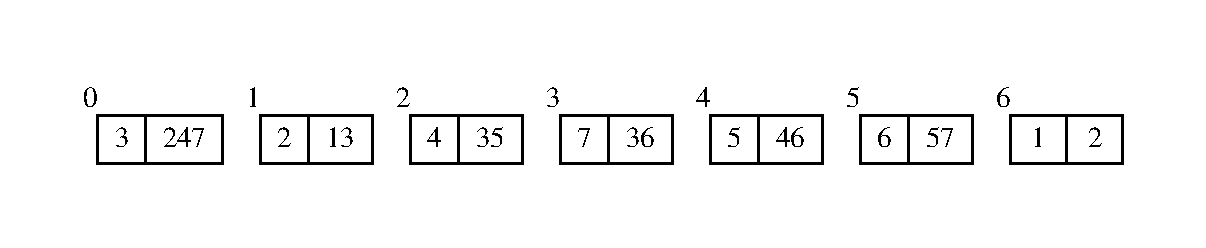
\includegraphics[scale=.6]{70-bute/img/leafysets}
  \caption{The STSs for our trie example}
  \label{fig:TrieSTSs}
\end{figure}

The trie is constructed element-by-element on line \codelineref{AddToSPrime}
of \Cref{ConstructingTheS}.  \Cref{fig:Trie} shows the trie after every element
of $\calS$ has been added.  For each set $S$, the trie stores $N(S)$,
sorted and represented as a string of vertices.
The shape of the trie is identical to that of a
Set-Trie \cite{DBLP:conf/IEEEares/Savnik13} with the $\{N(S) \mid S \in \calS'\}$
as elements.

\begin{figure}[htb]
  \newcommand{\TrieNode}[7]{\node (#1) [] at (#2) {
            \setlength{\tabcolsep}{2pt}
            \begin{tabular}{c c}
%                {\color{gray}$v$} & #3\\
                {\color{gray}$key$} & #4\\
                {\color{gray}$\bigwedge N(S)$} & #5\\
                {\color{gray}$\bigwedge S$} & #6
            \end{tabular}
        };}

  \newcommand{\STSNode}[4]{\node (#1) [stsnode] at (#2) {
            \setlength{\tabcolsep}{2pt}
            \begin{tabular}{c c}
                {\color{gray}$S$} & #3\\
                {\color{gray}$N(S)$} & #4
            \end{tabular}
        };}

  \centering
  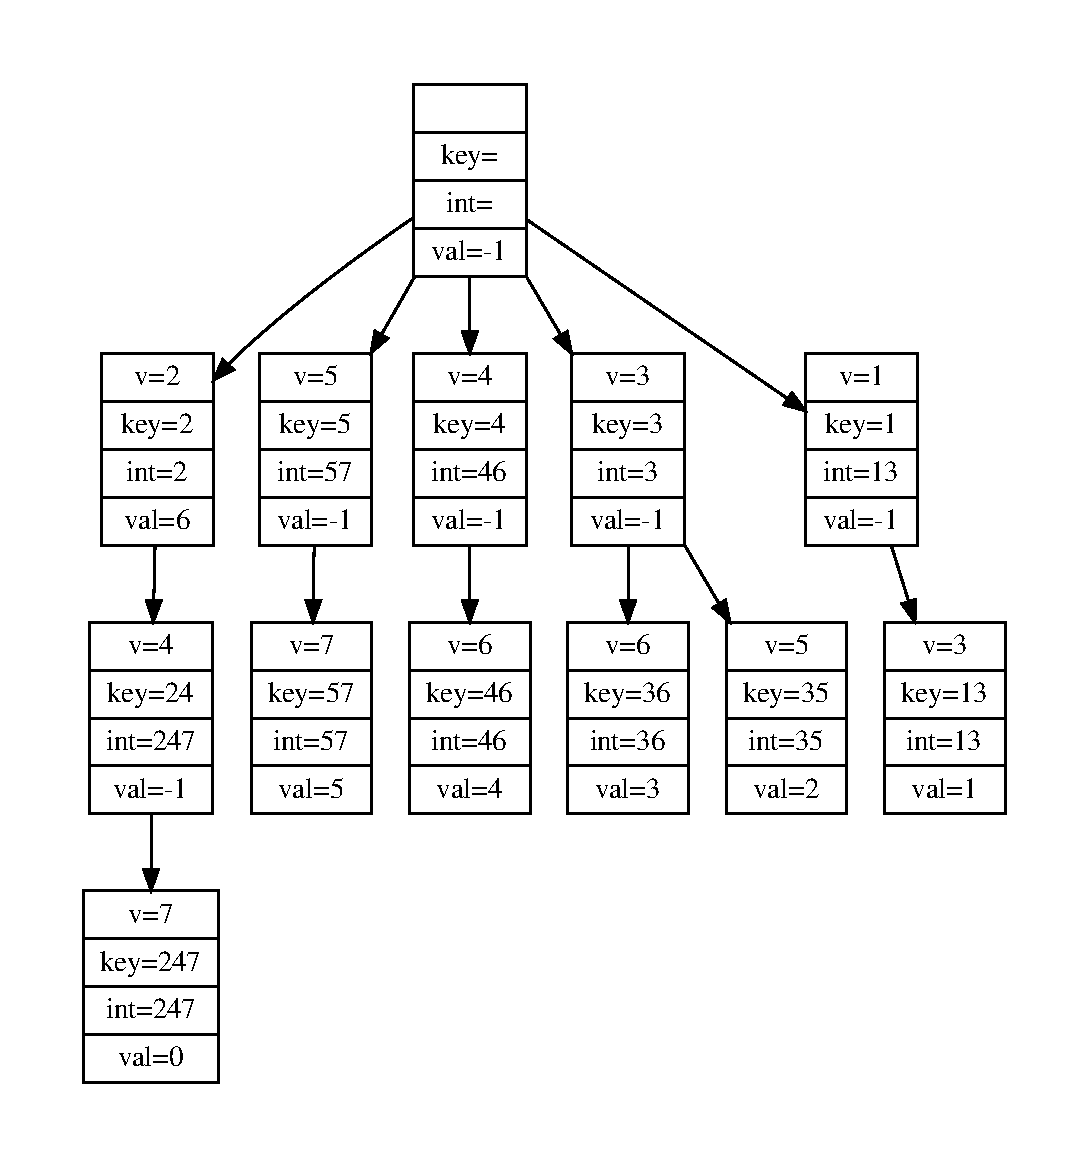
\includegraphics[scale=.5]{70-bute/img/trie}

    \begin{tikzpicture}[scale=0.85,
            every node/.style={scale=0.85, draw, shape=rectangle, black, inner sep=0pt, minimum size=14pt},
            stsnode/.style={draw=black, fill=black!15, shape=rectangle, rounded corners=5pt, inner sep=0pt, minimum size=14pt}]



  \TrieNode{noderoot}{4,0}{}{}{}{}{-1};
  \TrieNode{node0}{-1,-2.500000}{2}{2}{2}{}{6};
  \TrieNode{node1}{1,-2.500000}{5}{5}{57}{6}{-1};
  \TrieNode{node3}{3,-2.500000}{4}{4}{46}{5}{-1};
  \TrieNode{node5}{6,-2.500000}{3}{3}{3}{}{-1};
  \TrieNode{node8}{9,-2.500000}{1}{1}{13}{2}{-1};
  \TrieNode{node10}{-1,-5.000000}{4}{24}{247}{3}{-1};
  \TrieNode{node2}{1,-5.000000}{7}{57}{57}{6}{5};
  \TrieNode{node4}{3,-5.000000}{6}{46}{46}{5}{4};
  \TrieNode{node6}{5,-5.000000}{6}{36}{36}{7}{3};
  \TrieNode{node7}{7,-5.000000}{5}{35}{35}{4}{2};
  \TrieNode{node9}{9,-5.000000}{3}{13}{13}{2}{1};
  \TrieNode{node11}{-1,-7.500000}{7}{247}{247}{3}{0};
\STSNode{stsnode0}{-1,-9.5}{3}{247};
\STSNode{stsnode1}{9,-7}{2}{13};
\STSNode{stsnode2}{7,-7}{4}{35};
\STSNode{stsnode3}{5,-7}{7}{36};
\STSNode{stsnode4}{3,-7}{5}{46};
\STSNode{stsnode5}{1,-7}{6}{57};
\STSNode{stsnode6}{-3,-4.5}{1}{2};
\draw (noderoot.south) .. controls +(0,-.5) and +(0,.5) .. (node0.north);
\draw (noderoot.south) .. controls +(0,-.5) and +(0,.5) .. (node1.north);
\draw (noderoot.south) .. controls +(0,-.5) and +(0,.5) .. (node3.north);
\draw (noderoot.south) .. controls +(0,-.5) and +(0,.5) .. (node5.north);
\draw (noderoot.south) .. controls +(0,-.5) and +(0,.5) .. (node8.north);
\draw (node0.south) .. controls +(0,-.5) and +(0,.5) .. (node10.north);
\draw (node1.south) .. controls +(0,-.5) and +(0,.5) .. (node2.north);
\draw (node3.south) .. controls +(0,-.5) and +(0,.5) .. (node4.north);
\draw (node5.south) .. controls +(0,-.5) and +(0,.5) .. (node6.north);
\draw (node5.south) .. controls +(0,-.5) and +(0,.5) .. (node7.north);
\draw (node8.south) .. controls +(0,-.5) and +(0,.5) .. (node9.north);
\draw (node10.south) .. controls +(0,-.5) and +(0,.5) .. (node11.north);
\draw (node0.south) .. controls +(0,-.5) and +(0,.5) .. (stsnode6.north);
\draw (node2.south) .. controls +(0,-.5) and +(0,.5) .. (stsnode5.north);
\draw (node4.south) .. controls +(0,-.5) and +(0,.5) .. (stsnode4.north);
\draw (node6.south) .. controls +(0,-.5) and +(0,.5) .. (stsnode3.north);
\draw (node7.south) .. controls +(0,-.5) and +(0,.5) .. (stsnode2.north);
\draw (node9.south) .. controls +(0,-.5) and +(0,.5) .. (stsnode1.north);
\draw (node11.south) .. controls +(0,-.5) and +(0,.5) .. (stsnode0.north);
%        \TrieNode{root}{0,0}{}{}{}{-1};
%        \TrieNode{n0}{0,-2}{}{}{}{-2};
%
%%        \node (2) at (-1.2,1.2) {2};
%%        \node (3) at (-.3,1.2) {3};
%%        \node (4) at (.5,1.8) {4};
%%        \node (5) at (1.3,1.2) {5};
%%        \node (6) at (1,.3) {6};
%%        \node (7) at (0,.3) {7};
%%
%%        \draw (1) -- (2) -- (3) -- (4) -- (5) -- (6) -- (7) -- (3);
    \end{tikzpicture}
  \caption{A trie TODO describe this in some detail here; maybe a few lines. refer
  to the section of text}
  \label{fig:Trie}
\end{figure}

Each node of the trie has five elements:

\begin{itemize}
  \item \emph{key} is a set of vertices representing a neighbourhood
  \item \emph{v} is the vertex appended to the key of the parent node to give the key of the current node
  \item \emph{int} is the intersection of neighbourhoods of STSs stored in the subtrie rooted at this node
  \item \emph{val} is the index in the $\calS$ array (\Cref{fig:TrieSTSs} in our example) of the
    last element whose neighbourhood equals \emph{key}
  \item \emph{int'} (not shown in figure): the intersection of STSs stored in the subtrie rooted at this node
\end{itemize}

\subparagraph*{Querying the trie.} To query the data structure, we traverse the trie depth-first.
For a given $U$ and $i$, we wish to find all stored sets $S$ such that 
$|N(S) \cup N(U)| \leq i \wedge N[U] \cap S = \emptyset$.  There is
no need to visit a node $n$ or its descendants if either $|int(n) \cap N(U)| > i$
or $|N[u] \cap int'(n)| \not= \emptyset$. 

TODO: describe scanning in array after hitting a val

\subparagraph*{Inserting.} To insert a set $S$ into the trie, traverse the trie
depth-first, visiting only those nodes whose key is a prefix of $N(S)$.
When a node is reached none of whose children's key is a prefix of $N(S)$,
create a child and visit the child.  When you reach a node whose key is $N(S)$,
create an STS-node child.  As you go down the tree, modify the $Nint$ and $Sint$
fields by intersecting with $N(S)$ and $S$.
(?? say what the time complexity of insertion is)

We have implemented an additional small optimisation to the trie: in each node,
we store the number of values in the subtrie rooted at that node, along with
one of these values.  This allows us, at query time, to avoid the effort of traversing
all the way down to a leaf if there is only one value in the subtrie rooted
at the current node.  We emphasise that our trie has been implemented in a very
simple way, and that it is likely to be possible to optimise both speed and memory
use further.  For example, it would be possible to reduce space use by not explicitly storing
the descendants of a node with only one value in its subtrie.

\section{Improvements to the algorithm}\label{sec:improvements}

This section introduces two improvements the the algorithm that we have described so far:
domination rules and early stopping rules.

\subsection{Domination rule}

The Bute algorithm uses a domination-breaking rule that extends a rule
by Ganian et al.\ \cite{DBLP:conf/alenex/GanianLOS19,DBLP:journals/corr/abs-1911-12995}.
It is always
possible to construct an optimal elimination tree
such that for distinct vertices $v,w$ with 
$N(v) \setminus \{w\} \supset N(w) \setminus \{v\}$
we have that $w$ is not an ancestor of $v$.
Furthermore, if $N(v) \setminus \{w\} = N(w) \setminus \{v\}$
we can break symmetries by only allowing $w$ to be an ancestor
of $v$ if $v < w$.
TODO define \emph{dominates} here

Ganian et al.\ \cite{DBLP:conf/alenex/GanianLOS19,DBLP:journals/corr/abs-1911-12995}
describe a similar rule in the context of their partition-based SAT encoding,
but apply it only to the case where $v$ and $w$ are adjacent and do not specify
how the rule should be applied in the case where $u$ and $v$ have the same degree.

\subsubsection{How we use the rule in our algorithm}

We redefine the $\calS_i^k$ sets by adding two extra conditions.
Set $S$ can only be a member of $\calS_i^k$ if $S$ admits an elimination
tree of depth at most $k-i+1$ \emph{that respects the domination rule},
and if no vertex in $N(S)$ is dominated by a vertex in $S$.

TODO: write this properly.

1. Reject an STS if root dominates any adjacent vertices to STS.

2. Reject an STS if root is dominated by anything else in the STS.

3. Reject a possible root $v$ if the potential sub-STSs don't cover all of the
   adjacent dominated vertices of $v$.  TODO: probably move this
   to below the main proof below, since it's just an optimisation.
   But still prove it.

4. Reject a single-vertex STS $\{v\}$ if its neighbourhood contains
   any vertices domainated by $v$

??. Idea: how about adding an extra condition that if $N(S)$ is as big
    as can be, we can reject $S$ if any of its neighbours are adjacent to
    and dominated by vertices that are neither in $S$ nor $N(S)$?

Proof that this is correct:

Suppose $S \in \calS_i^k$.  We want to show that the algorithm will
generate $S$ by combining members of $\calS_{i+1}^k$ or by producing
a single-vertex set.  For the single-vertex case, it is clearly correct
(check this).  Otherwise, there is an elimination tree of $G[S]$
of depth TODO that respects the domination rule.  Its subtrees rooted at
depth 2 must also respect the domination rule.  TODO finish this paragraph.

We also need to show that every time the algorithm generates a set,
that it really fulfils the requirements for a member of $\calS_i^k$.
TODO finish this paragraph.

\subsubsection{Example of domination rule}

In the graph $G$ in \Cref{fig:examplegraph6}, vertex 1 dominates every other
vertex and vertex 6 is dominated by every other vertex.  Thus, there exists a
minimum-height elimination tree of $G$ that has 1 as the root and 6 as a leaf;
the second part of \Cref{fig:examplegraph6} shows such an elimination tree.
The algorithm rejects any STS containing 1 except... (?? say more), and also
rejects any STS with 6 as the root, except the single-vertex STS $\{6\}$.

\subsubsection{Proof of domination rule}

We now prove the correctness of the domination rule.
Given a graph $G$ and distinct vertices $v, w \in V(G)$
(with no restriction on whether $v$ and $w$ are adjacent),
we say that $v$ \emph{dominates} $w$
in $G$ if either of the following conditions holds:

\begin{itemize}
  \item $N(v) \setminus \{w\} \supset N(w) \setminus \{v\}$; or
  \item $N(v) \setminus \{w\} = N(w) \setminus \{v\}$ and $v > w$.
\end{itemize}

We use the notation $G[S]$ to denote the subgraph of $G$ induced by
vertex-set $S$, and $T[v]$ to denote the subtree of $T$ rooted at vertex
$v$.

\begin{theorem}
Let a connected graph $G$ be given.  There exists an elimination
tree $T$ of $G$ whose depth equals the treedepth of $G$, such
that for every vertex $w \in V(G)$ and every vertex $v \in V(G)$ that
dominates $w$ in $G$ we have that $w$ is not an ancestor of $v$ in $T$.
\end{theorem}

\begin{proof}
For ease
of exposition, we assume that the vertices of $G$ are numbered in nondecreasing
order of degree
(i.e. $v < w \implies |N(v)| \leq |N(w)|$), but the proof can easily be generalised
by defining an appropriate ordering relation on the vertices.

For an elimination tree $T$ of $G$, we define the \emph{score}
function $s_T : V(G) \mapsto \mathbb N \times V(G)$ that maps each
vertex $v$ to the tuple $(d,v)$ where $d$ is the depth of $v$ in $T$.
We compare scores lexicographically; thus, $v$ has a higher score than $v'$
if $v$ appears deeper in the tree than $v'$ or if the two vertices are at
the same depth and $v > v'$.  We also define the score of a tree: the score
of $T$ equals the minimum $s_T(v)$ over all vertices $v$ that are dominated
by one of their descendants.  If no such $v$ exists, the score of $T$
is the special value $(\infty, \infty)$.

%Suppose that every minimum-depth elimination tree $T$ of $G$
%breaks the domination rule; that
%is, there exist $v,v' \in V(G)$ such that $v$ dominates $v'$ in $G$ and
%$v'$ is an ancestor of $v$ in $T$.  Let
%$(d,u)$ be the maximum score of any minimum-depth elimination tree of $G$, and
%let $T$ be a minimum-depth elimination tree with this score.
%Let $w$ be the greatest-numbered vertex in $T[u]$ that dominates $u$.
%The subtree $T[u]$ may be replaced with an elimination tree that has the
%same vertex set as $T[u]$ but is rooted at $w$, without increasing the height of the
%subtree (since $G[V(T[u]) \setminus \{w\}]$
%is isomorphic to a subgraph of $G[V(T[u]) \setminus \{u\}]$).
%This replacement results in new elimination tree $T'$ of depth equal
%to the treedepth of $G$. The score of $T'$ is
%at least $(d, w)$, which is greater than $(d,u)$.
Let a minimum-depth elimination tree $T$ of $G$ that breaks the domination
rule be given; that
is, there exist $v,v' \in V(G)$ such that $v$ dominates $v'$ in $G$ and
$v'$ is an ancestor of $v$ in $T$.
We will demonstrate that it is possible to reorder a subtree of $T$ to obtain
a new minimum-depth elimination tree of strictly greater score than $T$.  Repeated
application of this rule must yield a minimum-depth elimination tree that
does not break the domination rule, since there are only finitely many
different scores that elimination trees of a finite graph can have.

Let $(d,u)$ be the score of $T$.
Let $w$ be the greatest-numbered vertex in $T[u]$ that dominates $u$.
The subtree $T[u]$ may be replaced with an elimination tree that has the
same vertex set as $T[u]$ but is rooted at $w$, without increasing the height of the
subtree (since $G[V(T[u]) \setminus \{w\}]$
is isomorphic to a subgraph of $G[V(T[u]) \setminus \{u\}]$).
This replacement results in new minimum-depth elimination tree $T'$ of
$G$. The score of $T'$ is at least $(d, w)$, which is greater than $(d,u)$.
\end{proof}

\subsection{Early stopping rules}

Rule 1: On some instances (such as PACE 2020 exact instance 047), we can save quite a bit of work
on the satisfiable instance of the decision problem using the following rule.  After
generating the set $\calS_i^k$, the algorithm tests for each $S \in \calS_i^k$
whether $S \cup N(S) = V(G)$.  If this condition holds, then clearly we can form
an elimination tree by beginning with an elimination tree $T$ of $S$, then adding any vertex
$v \in N(S)$ as the parent of the root of $T$, and continuing to add each vertex
in $N(S)$ (in any order) as the parent of the current root.

Rule 2: if $S_i^k$ does not introduce any new sets, we can quit.  Prove this.  Or probably
better just to remove this rule from the code?

\section{Implementation details}\label{sec:implementation}

We wrote the code in C.

We store sets of vertices using bitsets.  We have implemented the most common operations
on these, such as computing the number of elements in the union of two bitsets.  This
means that although operations are $O(|V(G)|)$, they are very fast in practice.

We implemented a hash map with bitsets as keys and integers as values.
This is used for storing the root vertex of each subtree-set.  We also use the map data
structure to store sets of bitsets.

Optimisations to trie.

Store neighbourhood with STS for speed.

\section{How does the Bute algorithm differ from other entries to the exact track of PACE 2020?}\label{sec:paceentries}

Tom van der Zanden's algorithm (\url{https://github.com/TomvdZanden/BasicTreedepthSolver})
looks very similar to mine.  I reckon he's come up with pretty much the same idea, and he
even says that you could use a Trie to speed it up, but he doesn't give details.  He doesn't
use domination rules.

PID* (\url{https://github.com/maxbannach/PID-Star}), by Max Bannach and others,
seems to use a similar approach.  It uses a priority queue, a bit like A* search; my understanding
is that could save quite a bit of time on the satisfiable decision problem.  It also adds some
preprocessing rules, some of which I could probably add to my algorithm.
They have a 2019 paper which I still don't understand, but which seems to outline
part of their method using game-theoretic language which I find very difficult to get
my head around \cite{DBLP:conf/wads/BannachB19}.  So I'll need to try to relate my
algorithm to their earlier work.

And I've just come across \url{https://zenodo.org/record/3894555} by Bojikian and others.
Yikes!  From a quick look, it seems to do \emph{very} similar things to my algorithm.
Maybe it's even exactly the same algorithm!  But it doesn't perform very well in practice,
so their implementation is maybe not very good (they solve 69 PACE Challenge instances
within the 30 minute time limit, whereas we solve 80).

swats's solver is a heuristic that just happens to give correct answers for the public
instances.

The other three leading solvers use a top-down approach, generating minimal separators.
I still haven't looked closely at their details, but they are very different from the approach
we're presenting in this paper.  Their approach is much more like my SEA 2020 paper, but they
do much better than my algorithm.

\section{Experiments}\label{sec:experiments}

\subsection{Beauty contest}

TODO: which types of instances is it good and bad at solving?

\begin{figure}[htb]
  \centering
  PLOT GOES HERE
  \caption{Run times of SMS and Bute on the PACE Challenge private instances.}
  \label{fig:runtimes}
\end{figure}

\subsection{How much memory does it use? / How many sets does it store as instance size grows?}

\subsection{How does it scale compared to other algorithms?}

\section{Conclusion}\label{sec:conclusion}

We have introduced an exact, exponential-time and -space algorithm for the treedepth problem
that solves in a bottom-up, dynamic-programming, PID (I think) style.  Our experiments show that
it performs similarly overall to the SMS algorithm by ?? which was also submitted to the PACE Challenge,
although neither solver dominates the other on all the instances.   SMS is a very different type
of solver (top-down rather than bottom-up), so it's nice to see that both approaches are viable
and that they each seem to have their strengths.

We can probably improve Bute further by borrowing some techniques, such as preprocessing
steps, from Ganian et al.\ and from the other PACE Challenge solvers.
